\documentclass[11pt,class=report,crop=false]{standalone}
\usepackage[screen]{../python}

\begin{document}

%====================================================================
\chapitre{Constructions aléatoires}
%====================================================================

\objectifs{Tu vas programmer deux méthodes pour construire des figures qui ressemblent à des algues ou des coraux. Chaque figure est formée de petits blocs lancés au hasard et qui se collent les uns aux autres.}

\begin{center}
\begin{minipage}{0.4\textwidth}
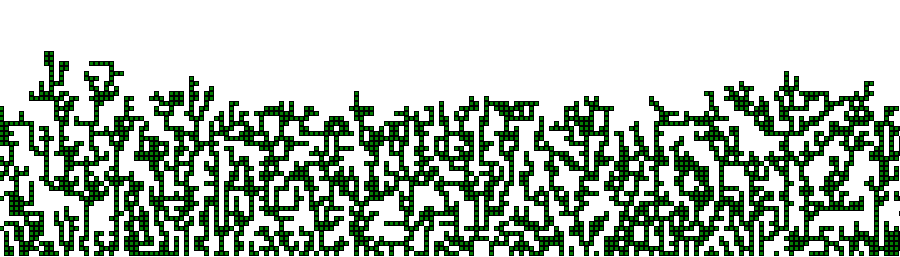
\includegraphics[scale=\myscale,scale=0.3]{ecran-alea-bloc00}
\end{minipage}
\begin{minipage}{0.3\textwidth}
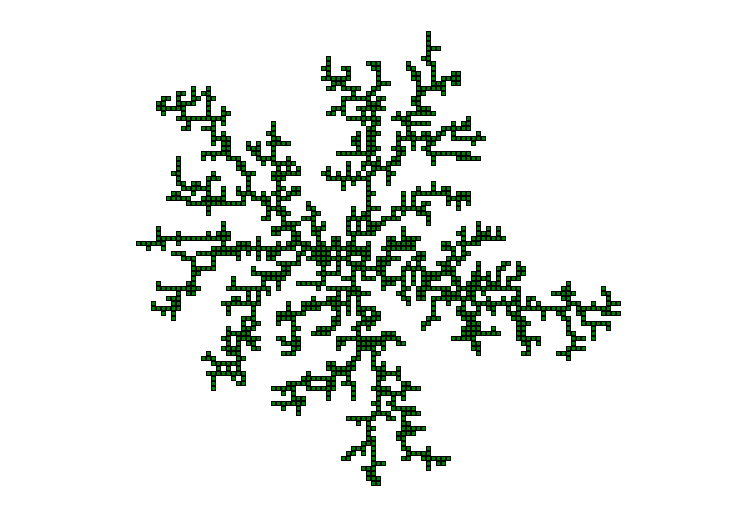
\includegraphics[scale=\myscale,scale=0.25]{ecran-alea-arbre00}
\end{minipage}
\end{center}


\insertvideo{-AgiGtmzvI0}{Constructions aléatoires}

\insertvideo{DJWA7bFiimA}{Mouvement avec tkinter}


%%%%%%%%%%%%%%%%%%%%%%%%%%%%%%%%%%%%%%%%%%%%%%%%%%%%%%%%%%%%%%%%
%%%%%%%%%%%%%%%%%%%%%%%%%%%%%%%%%%%%%%%%%%%%%%%%%%%%%%%%%%%%%%%%

\begin{cours}[Chutes de blocs]
On fait tomber des blocs carrés dans une grille, sur le principe du jeu \og{}Puissance 4\fg{} : après avoir choisi une colonne, un bloc tombe du haut vers le bas. Les blocs se posent sur le bas de la grille ou sur des autres blocs ou à côté d'autres blocs. Il y a une grosse différence avec le jeu \og{}Puissance 4\fg{}, ici les blocs sont \og{}collants\fg{}, c'est-à-dire qu'un bloc reste collé dès qu'il rencontre un voisin à gauche ou à droite.


Voici un exemple de lancer de blocs :
\myfigure{0.5}{
\footnotesize
  \tikzinput{fig-alea-bloc0}
}

Par exemple à l'étape 4, le bloc lancé dans la colonne numéro $2$ ne descend pas jusqu'en bas mais reste \og{}scotché\fg{} à son voisin, il se retrouve donc définitivement suspendu.

Le lancer aléatoire de centaines de blocs sur une grande grille produit de jolies formes géométriques ressemblant à des algues.

\begin{center}
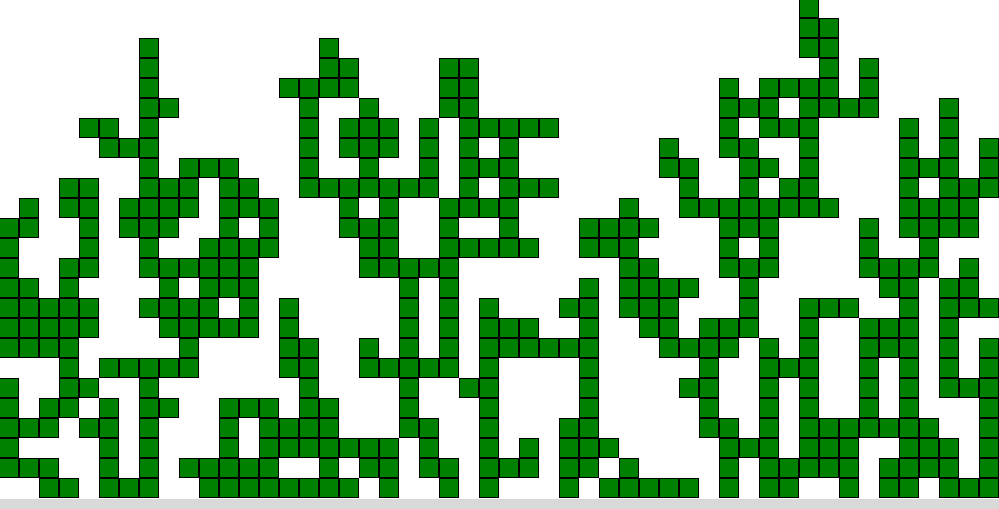
\includegraphics[scale=\myscale,scale=0.3]{ecran-alea-bloc0}
\end{center}

\end{cours}



%%%%%%%%%%%%%%%%%%%%%%%%%%%%%%%%%%%%%%%%%%%%%%%%%%%%%%%%%%%%%%%%
% Activité 1 - Chutes de blocs
%%%%%%%%%%%%%%%%%%%%%%%%%%%%%%%%%%%%%%%%%%%%%%%%%%%%%%%%%%%%%%%%

\begin{activite}[Chutes de blocs]

\objectifs{Objectifs : programmer la chute des blocs (sans affichage graphique).}

On modélise l'espace de travail par un tableau de $n$ lignes et $p$ colonnes. Au départ le tableau ne contient que des $0$ ;
 ensuite la présence d'un bloc est représentée par $1$.

Voici comment initialiser le tableau :\\
\centerline{\ci{tableau = [[0 for j in range(p)] for i in range(n)]}}
On modifie le tableau par des instructions du type :\\
\centerline{\ci{tableau[i][j] = 1}}


Voici un exemple de tableau (à gauche) pour représenter la situation graphique de droite (le bloc en haut à droite est en train de tomber).

\begin{center}
\begin{minipage}{0.3\textwidth}
$$\begin{array}{cccccc}
0&0&0&0&1&0\\
0&0&1&0&0&0\\
0&0&1&0&0&0\\
0&0&1&1&0&0
\end{array}$$
\end{minipage}
\begin{minipage}{0.4\textwidth}
\myfigure{0.7}{
  \tikzinput{fig-alea-bloc1}
}
\end{minipage}
\end{center}

\begin{enumerate}
  \item Programme une fonction \ci{peut_tomber(i,j)} qui détermine si le bloc en position $(i,j)$ peut descendre d'une case ou pas.
  
  Voici les cas dans lesquels le bloc \emph{ne peut pas} tomber :
  \begin{itemize}
    \item si le bloc est déjà sur la dernière ligne,
    \item s'il y a un bloc juste en dessous,
    \item s'il y a un bloc juste à droite ou juste à gauche.
  \end{itemize}
  
  \item Programme une fonction \ci{faire_tomber_un_bloc(j)}
qui fait tomber un bloc dans la colonne $j$ jusqu'à ce qu'il ne puisse plus descendre.
Cette fonction modifie les entrées du tableau.  
  
  Par exemple, voici le tableau avant (à gauche) et après (à droite) avoir fait tomber un bloc dans la colonne $j=3$.  
  
$$\begin{array}{cccccc}
0&0&0&0&0&0\\
0&0&1&0&0&0\\
0&0&1&0&0&0\\
0&0&1&1&0&0
\end{array}\qquad\qquad
\begin{array}{cccccc}
0&0&0&0&0&0\\
0&0&1&1&0&0\\
0&0&1&0&0&0\\
0&0&1&1&0&0
\end{array}
$$
 
 \myfigure{0.7}{
  \tikzinput{fig-alea-bloc2}
} 

 
  \item Programme une fonction \ci{faire_tomber_des_blocs(k)} qui lance 
  $k$ blocs un par un, en choisissant à chaque fois une colonne au hasard (c'est-à-dire un entier $j$ avec $0 \le j < p$). 
  
  Voici un exemple de tableau obtenu après avoir lancé $10$ blocs :
  
 
\begin{center}
\begin{minipage}{0.3\textwidth} 
 $$\begin{array}{cccccc} 
0&0&0&1&1&0\\
0&1&1&1&0&0\\
0&0&1&0&0&1\\
0&0&1&1&0&1
\end{array}
$$
\end{minipage}
\begin{minipage}{0.4\textwidth} 
 \myfigure{0.7}{
  \tikzinput{fig-alea-bloc3}
} 
\end{minipage}
\end{center}  

\end{enumerate}

\end{activite}


%%%%%%%%%%%%%%%%%%%%%%%%%%%%%%%%%%%%%%%%%%%%%%%%%%%%%%%%%%%%%%%%
% Activité 2 - Chutes de blocs
%%%%%%%%%%%%%%%%%%%%%%%%%%%%%%%%%%%%%%%%%%%%%%%%%%%%%%%%%%%%%%%%

\begin{activite}[Chutes de blocs (suite)]

\objectifs{Objectifs : programmer l'affichage graphique des blocs.}

\textbf{Affichage statique.} Programme l'affichage graphique des blocs à partir d'un tableau.

\begin{center}
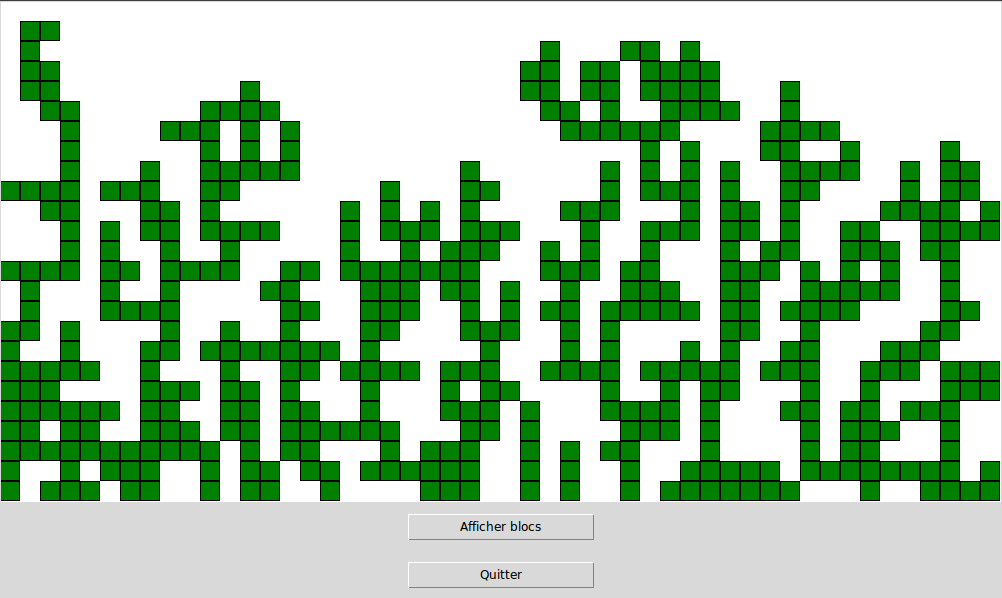
\includegraphics[scale=\myscale,scale=0.3]{ecran-alea-bloc1}
\end{center}
\medskip

\emph{Indications.}
\begin{itemize}
  \item Utilise le module \ci{tkinter}, voir la fiche \og{}Statistique -- Visualisation de données\fg{}.
  \item Tu peux rajouter un bouton qui lance un bloc (ou plusieurs d'un coup). 
\end{itemize}

\medskip



\textbf{Affichage dynamique (facultatif et difficile).} Programme l'affichage des blocs qui tombent.
\medskip

\begin{center}
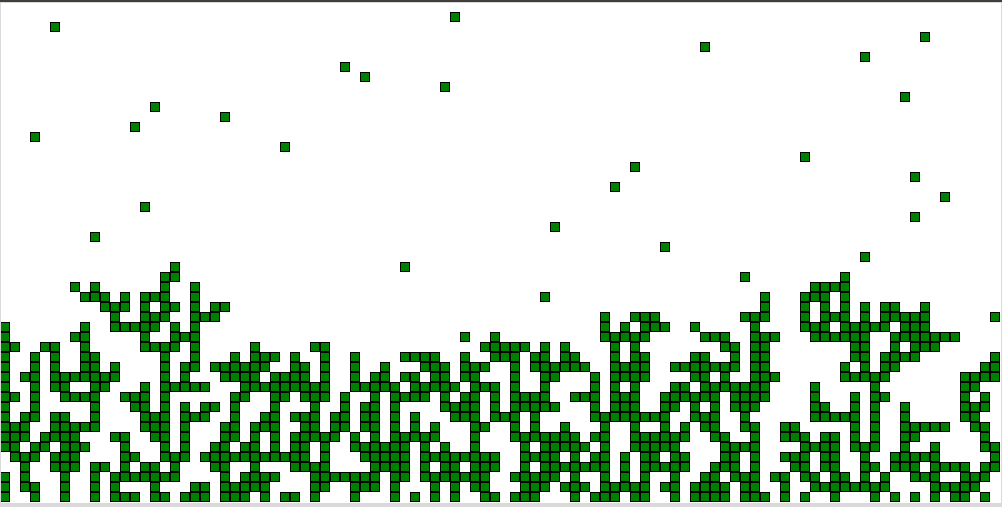
\includegraphics[scale=\myscale,scale=0.3]{ecran-alea-bloc2}
\end{center}

\emph{Indications.} 
\begin{itemize}
  \item C'est beaucoup plus compliqué à programmer, mais très joli à voir ! 
  \item Pour le déplacement des blocs, inspire-toi du programme \og{}Mouvement avec \ci{tkinter}\fg{} à la fin de cette fiche.
  \item Pour faire une \og{}pluie de blocs\fg{} de façon régulière (par exemple tous les dixièmes de secondes) : on fait descendre tous les blocs existant d'une case et on en fait apparaître un nouveau sur la ligne du haut.
\end{itemize}
\end{activite}





%%%%%%%%%%%%%%%%%%%%%%%%%%%%%%%%%%%%%%%%%%%%%%%%%%%%%%%%%%%%%%%%
%%%%%%%%%%%%%%%%%%%%%%%%%%%%%%%%%%%%%%%%%%%%%%%%%%%%%%%%%%%%%%%%

\begin{cours}[Arbres browniens]

Voici une construction un peu différente, beaucoup plus longue à calculer, mais qui dessine aussi de jolies figures appelées \og{}arbres browniens\fg{}.

\begin{center}
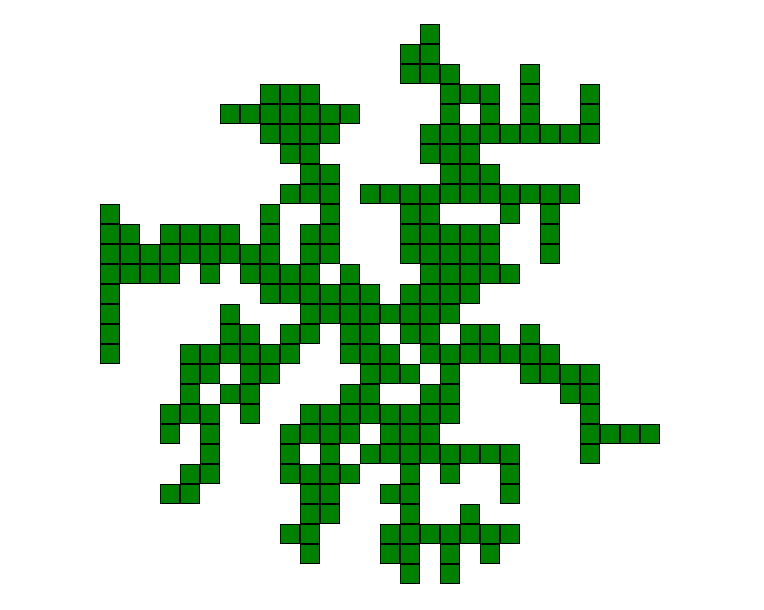
\includegraphics[scale=\myscale,scale=0.28]{ecran-alea-arbre1}
\end{center}


Le principe est le suivant :
\begin{itemize}
  \item On part d'une grille (il faut cette fois imaginer qu'elle est dessinée à plat sur une table). En son centre, on place un premier bloc fixe, le \emph{germe}.
  
  \item On fait apparaître un bloc au hasard sur la grille. À chaque étape, ce bloc se déplace au hasard sur l'une des huit cases adjacentes, on parle d'un \emph{mouvement brownien}. 

  \item Dès que ce bloc touche un autre bloc par un côté, il s'y colle et ne bouge plus.

  \item Si le bloc sort de la grille, il se désintègre.
  
  \item Une fois le bloc collé ou désintégré, on relance alors un nouveau bloc depuis un point aléatoire de la grille.
\end{itemize}


\myfigure{0.5}{
\footnotesize
  \tikzinput{fig-alea-arbre1}
} 

On obtient petit à petit une sorte d'arbre qui ressemble à du corail. Les calculs sont très longs car beaucoup de blocs sortent de la grille ou mettent longtemps avant de se fixer (surtout au début). En plus, on ne peut lancer les blocs qu'un par un.

\end{cours}



%%%%%%%%%%%%%%%%%%%%%%%%%%%%%%%%%%%%%%%%%%%%%%%%%%%%%%%%%%%%%%%%
% Activité 3 - Arbres browniens
%%%%%%%%%%%%%%%%%%%%%%%%%%%%%%%%%%%%%%%%%%%%%%%%%%%%%%%%%%%%%%%%

\begin{activite}[Arbres browniens]

\objectifs{Objectifs : programmer la création d'un arbre brownien.}

\textbf{Première partie.}

\begin{enumerate}
  \item Modélise de nouveau l'espace de travail par un tableau de $n$ lignes et $p$ colonnes contenant des $0$ ou des $1$. Initialise toutes les valeurs à $0$ sauf $1$ au centre du tableau.
  
  \item Programme une fonction \ci{est_dedans(i,j)} qui détermine si la position $(i,j)$ est bien dans la grille (sinon c'est que le bloc est en train de sortir).
    
  \item  Programme une fonction \ci{est_libre(i,j)} qui détermine si le bloc en position $(i,j)$ peut bouger (la fonction renvoie \og{}vrai\fg{}) ou s'il est collé (la fonction renvoie \og{}faux\fg{}).

  \item Programme une fonction \ci{lancer_un_bloc()}, sans paramètre, qui simule la création d'un bloc et son déplacement aléatoire, jusqu'à ce qu'il se colle ou qu'il quitte la grille.
  
  \emph{Indications.}
  \begin{itemize}
    \item Le bloc est créé à une position aléatoire $(i,j)$ de la grille.
    \item Tant que le bloc est dans la grille et libre de bouger :
    \begin{itemize}
      \item tu choisis un déplacement horizontal en tirant au hasard un entier  parmi $\{-1,0,+1\}$, idem pour un déplacement vertical ;
      \item tu déplaces le bloc selon la combinaison de ces deux mouvements.
      \end{itemize}  
      \item Modifie alors le tableau.      
  \end{itemize}

  
    \item Termine avec une fonction \ci{lancer_des_blocs(k)} qui lance $k$ blocs.   
\end{enumerate}


\textbf{Seconde partie.}

Programme l'affichage graphique à l'aide de \ci{tkinter}. Tu peux ajouter un bouton qui lance $10$ blocs d'un coup.

\begin{center}
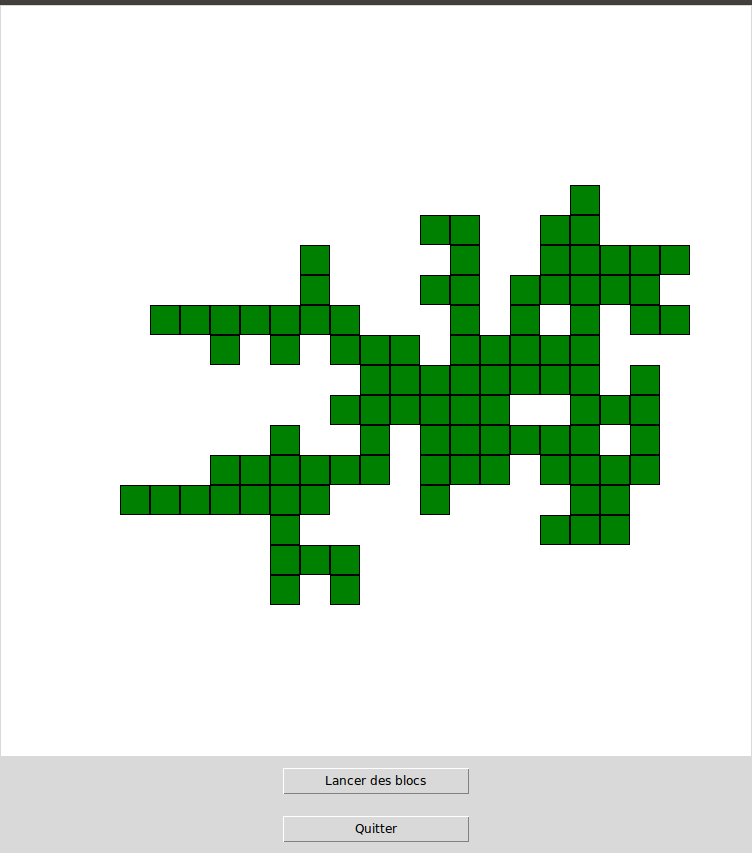
\includegraphics[scale=\myscale,scale=0.24]{ecran-alea-arbre2}
\end{center}

\end{activite}


%%%%%%%%%%%%%%%%%%%%%%%%%%%%%%%%%%%%%%%%%%%%%%%%%%%%%%%%%%%%%%%%
%%%%%%%%%%%%%%%%%%%%%%%%%%%%%%%%%%%%%%%%%%%%%%%%%%%%%%%%%%%%%%%%


\begin{cours}[Mouvement avec \og{}tkinter\fg{}]

\index{tkinter@\ci{tkinter}}
\index{module!tkinter@\ci{tkinter}}

Voici un programme qui fait se déplacer un petit carré et le faisant rebondir sur les bords de la fenêtre.

\begin{center}
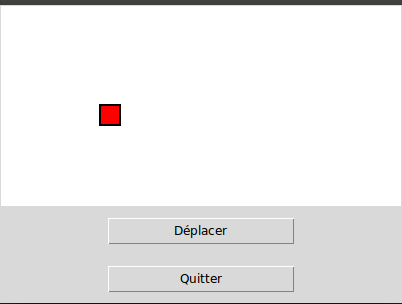
\includegraphics[scale=\myscale,scale=0.5]{ecran-alea-cours-mouv}
\end{center}

Voici les points principaux :
\begin{itemize}
  \item Un objet \ci{rect} est défini, c'est une variable globale, de même que ses coordonnées \ci{x0}, \ci{y0}.
  
  \item Cet objet est (un petit peu) déplacé par la fonction \ci{deplacer()} qui décale le rectangle de \ci{(dx,dy)}.
    
  \item Le point clé est que cette fonction sera exécutée une nouvelle fois après un court laps de temps. La commande :\\
  \centerline{\ci{canvas.after(50,deplacer)}}
  demande une nouvelle exécution de la fonction \ci{deplacer()} après un court délai (ici $50$ millisecondes).
  
  \item La répétition de petits déplacements simule le mouvement.
\end{itemize}

\begin{lstlisting}
from tkinter import *

Largeur = 400
Hauteur = 200

root = Tk()     
canvas = Canvas(root, width=Largeur, height=Hauteur, background="white")
canvas.pack(fill="both", expand=True)

# Les coordonnées et la vitesse
x0, y0 = 100,100
dx = +5  # Vitesse horizontale
dy = +2  # Vitesse verticale

# Le rectangle à déplacer
rect = canvas.create_rectangle(x0,y0,x0+20,y0+20,width=2,fill="red")

# Fonction principale
def deplacer():
    global x0, y0, dx, dy

    x0 = x0 + dx  # Nouvelle abscisse
    y0 = y0 + dy  # Nouvelle ordonnée

    canvas.coords(rect,x0,y0,x0+20,y0+20)  # Déplacement

    if x0 < 0 or x0 > Largeur:
        dx = -dx  # Changement de sens horizontal
    if y0 < 0 or y0 > Hauteur:
        dy = -dy  # Changement de sens vertical

    canvas.after(50,deplacer)  # Appel après 50 millisecondes
 
    return
    
# Fonction pour le bouton
def action_deplacer():
    deplacer()
    return

# Boutons
bouton_couleur = Button(root,text="Déplacer", width=20, command=action_deplacer)
bouton_couleur.pack(pady=10)

bouton_quitter = Button(root,text="Quitter", width=20, command=root.quit)
bouton_quitter.pack(side=BOTTOM, pady=10)

root.mainloop()
\end{lstlisting}

\end{cours}

\end{document}
